\documentclass[a4paper]{book}
\usepackage[nottoc]{tocbibind}
\usepackage{graphicx}
\usepackage{amsmath,amsthm}
\usepackage{float}
\usepackage{geometry}
\usepackage{listings}
\usepackage{multicol}
\usepackage{relsize}
\usepackage{float}
\usepackage{caption}
\usepackage{enumitem}
\usepackage{amssymb}
\usepackage{tikz,pgfplots}
\usepackage[pagebackref=false,colorlinks,linkcolor=blue,citecolor=blue,urlcolor=cyan]{hyperref}
\usepackage[americanvoltages,fulldiodes,siunitx]{circuitikz}
\usepackage{wrapfig}
\usepackage{amsfonts}
\usepackage{mathtools}
\usepackage{bbm}
\usepackage{multicol}
\usepackage{titlesec}
\usepackage{hyperref}
\usepackage{amsmath}
\usepackage{listings}
\usepackage{algorithm}
\usepackage{algorithmic}
%\usepackage{algpseudocode}
\usetikzlibrary{decorations.pathmorphing,patterns}
\geometry{
	a4paper,
	total={164mm,247mm},
	left=23mm,
	top=25mm,
}
\usepackage{listings}
\usepackage{xcolor}
\usepackage{subcaption}
\definecolor{mGreen}{rgb}{0,0.6,0}
\definecolor{mGray}{rgb}{0.5,0.5,0.5}
\definecolor{mPurple}{rgb}{0.58,0,0.82}
\definecolor{backgroundColour}{rgb}{0.95,0.95,0.92}

\DeclareMathOperator*{\p}{\mathbb{P}} 
\DeclareMathOperator*{\e}{\mathbb{E}} 
\DeclareMathOperator*{\privk}{\mathrm{PrivK}_{\A,\Pi}^\mathrm{eav}} 
\DeclareMathOperator*{\privkk}{\mathrm{PrivK}_{\mathcal{\bar{A}},\Pi}^\mathrm{eav}}
\DeclareMathOperator*{\D}{\mathcal{D}} 
\DeclareMathOperator*{\A}{\mathcal{A}} 
\DeclareMathOperator*{\B}{\mathcal{B}} 
\DeclareMathOperator*{\R}{\mathbb{R}} 
\DeclareMathOperator*{\GG}{\mathbb{G}} 
\DeclareMathOperator*{\ZZ}{\mathbb{Z}} 
\DeclareMathOperator*{\Enc}{\mathsf{Enc}} 
\DeclareMathOperator*{\Dec}{\mathsf{Dec}} 
\DeclareMathOperator*{\Vrfy}{\mathsf{Vrfy}} 
\DeclareMathOperator*{\Mac}{\mathsf{Mac}} 
\DeclareMathOperator*{\Abar}{\mathcal{\bar{A}}} 
\DeclareMathOperator*{\F}{\mathcal{F}} 
\DeclareMathOperator*{\RR}{\mathbb{R}} 
\DeclareMathOperator*{\bW}{\mathbf{W}} 
\DeclareMathOperator*{\bB}{\mathbf{B}} 


\titleformat{\section}
{\normalfont\fontsize{20}{20}\bfseries}{\thesection}{1em}{}

\titleformat{\subsection}
{\normalfont\fontsize{15}{20}\bfseries}{\thesubsection}{1em}{}

\titleformat{\subsubsection}
{\normalfont\fontsize{12}{20}\bfseries}{\thesubsubsection}{1em}{}

\usepackage{fancyhdr}
\pagestyle{fancy}
\fancyhf{}

%%%%%%%%%%%%%%%%%%%
\rhead{مقدمه‌ای بر محرمانگی تفاضلی}

\lhead{گروه مطالعاتی دکتر جواد ابراهیمی}
%%%%%%%%%%%%%%%%%%%


%\cfoot{(\space \space \space \space \textbf{\thepage}  \space \space \space)}
\cfoot{\thepage}
\renewcommand{\headrulewidth}{1pt}
%\renewcommand{\footrulewidth}{1pt}

\setlength{\parindent}{1.5em}
\setlength{\parskip}{0.9em}
\renewcommand{\baselinestretch}{1.4}


\newtheorem{theorem}{قضیه}
\newtheorem{annotation}{نمادگذاری}
\newtheorem{proposition}{گزاره}
\newtheorem{claim}{ادعا}
\newtheorem{lemma}{لم}
\newtheorem{corollary}{نتیجه}
\newtheorem{definition}{تعریف} % Use this for non-trivial definitions.

\newcommand\myeq{\mathrel{\stackrel{\makebox[0pt]{\mbox{\normalfont\tiny def}}}{=}}}


\usepackage{xepersian}
\settextfont{XB_NILOOFAR.ttf}
\setdigitfont{XB_NILOOFAR.ttf}

\makeatletter
\bidi@patchcmd{\@Abjad}{آ}{الف}
{\typeout{Succeeded in changing `آ` into `الف`}}
{\typeout{Failed in changing `آ` into `الف`}}
\makeatother
\PersianAlphs


\lstdefinestyle{CStyle}{
	backgroundcolor=\color{backgroundColour},   
	commentstyle=\color{mGreen},
	keywordstyle=\color{magenta},
	numberstyle=\tiny\color{mGray},
	stringstyle=\color{mPurple},
	basicstyle=\ttfamily,
	breakatwhitespace=false,         
	breaklines=true,                 
	captionpos=b,                    
	keepspaces=true,                 
	numbers=left,                    
	numbersep=5pt,                  
	showspaces=false,                
	showstringspaces=false,
	showtabs=false,                  
	tabsize=2,
	language=C
}

\lstdefinestyle{JavaStyle}{
	backgroundcolor=\color{backgroundColour},   
	commentstyle=\color{mGreen},
	keywordstyle=\color{magenta},
	numberstyle=\tiny\color{mGray},
	stringstyle=\color{mPurple},
	basicstyle=\footnotesize,
	breakatwhitespace=false,         
	breaklines=true,                 
	captionpos=b,                    
	keepspaces=true,                 
	numbers=left,                    
	numbersep=5pt,                  
	showspaces=false,                
	showstringspaces=false,
	showtabs=false,                  
	tabsize=2,
	language=java
}

\begin{document}
	\large
\begin{titlepage}
	
	\begin{center}
		\textbf{
			باسمه تعالی\\
		}
		\vspace{2cm}
		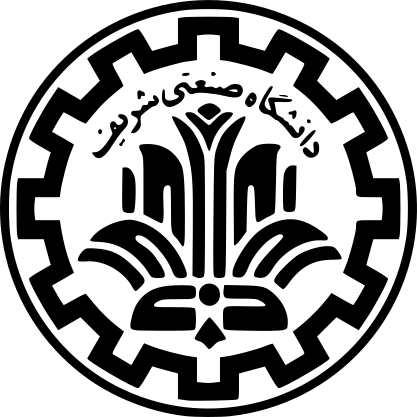
\includegraphics[scale=0.23]{logo.png}\\
		\vspace{0.5cm}
		\begin{Large}
			\textbf{
				دانشگاه صنعتی شریف\\
				\vspace{0.5cm}
				دانشکده ریاضی و علوم کامپیوتر\\
			}
			\vspace{2cm}			
		\end{Large}
		\begin{huge}
			\textbf{
			‌مقدمه‌ای بر محرمانگی تفاضلی و کاربردها  \\
		\LARGE{\LR{an Introduction to Differential Privacy and Applications}}
		\\
			}
		\end{huge}
		\vspace{5.5cm}
		\begin{Large}
			\textbf{
				گروه مطالعاتی دکتر جواد ابراهیمی بروجنی\\
				\vspace{.5cm}
				نگارنده: دانیال آیتی\\
				(و جمعی از دانشجویان گروه) \\
				\vspace{1cm}
				تابستان ۱۴۰۳
			}
		\end{Large}
	\end{center}
	\thispagestyle{empty}
\end{titlepage}	

\textbf{\huge
پیش‌گفتار
}
\vspace{.8cm}
\\

با توجه به مطرح شدن حوزه محرمانگی تفاضلی که حوزه‌ای بسیار جدید است و در عین حال داشتن تئوری ریاضی مشخص و فرمول‌بندی شده، به صورت مستقیم در صنعت کاربردهای فراوان دارد.
\\
\vspace{.4cm}

همجنین دانشجویان این گروه در تهیه و تنظیم و نوشتن این جزوه تلاش بسیاری کرده‌اند که از آنان تشکر ویژه به عمل می‌آوریم:
\\
علی‌رضا توفیقی محمدی - فیروزه ابریشمی - محمدحسین کلانتری - مهشید دهقانی - سارا کرمانی و مهدی عباس‌زاده
\\

\vspace{14cm}
امید است این کتابچه برای علاقه‌مندان و پژوهش‌گران مفید واقع شود.	
\tableofcontents
\chapter{مقدّمه}
 در ابتدا مقدمه‌ای از نیاز به محرمانگی در بسیاری از وقایع روزمره را بررسی می‌کنیم؛ که البته فعلا خالی از مطلب است!
 
\section{
امنیت و حریم خصوصی در زندگی مدرن
}

در ابتدا عکسی معروف که احتمالا در تمام جزوه‌ها دیدید را این‌جا قرار می‌دهم تا فرمت قرار دادن عکس را هم ببینید:
\newpage
\subsection{
مثال‌هایی از نیاز به محرمانگی و امنیت
}
اگر مسئله جایزه نتفلیکس
\footnote{\lr{Netflix prize}}
 را به خاطر داشته باشید، که تحول عظیمی در حوزه
 سیستم‌های پیشنهاددهنده
\footnote{\lr{Recommender Systems}}
به وجود آورد، جالب است بدانید که در یک تحقیق معروف که عکس آن در زیر قرار داده شده‌است، به این نتیجه رسیدند که داده‌هایی که برای این مسابقه در اختیار عموم قرار داده شده‌اند (که داده‌های واقعی بودند.)، هنگامی که در کنار داده‌های جمع شده از نظرات سایت معروف
\lr{IMDb}
قرار بگیرند، می‌تواند منجر به لو رفتن اطلاعات کاربران شوند. با داشتن نظرات تعداد محدودی کاربر در مورد تعداد مشخصی فیلم، می‌توان جدول یکتایی برای نظر هرکاربر نسبت به هر فیلم ارائه داد، البته توجه کنید این پارگراف را بدون هیچ دلیلی نوشته‌ام و فقط برای آماده کردن تمپلیت بود!

\begin{figure}[h]
	\centering
	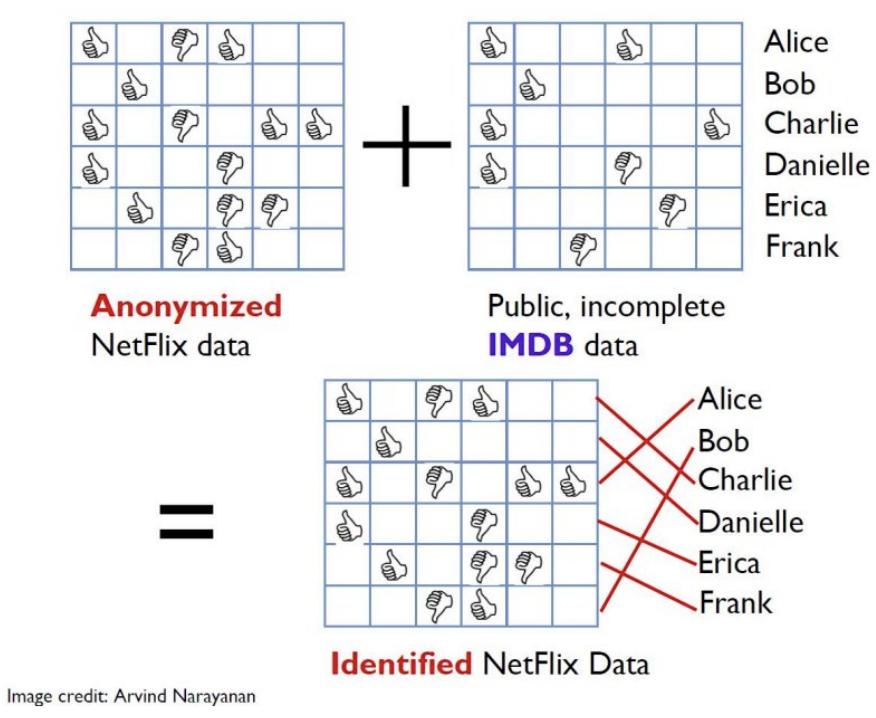
\includegraphics[width=0.6\linewidth]{Introduction/netflix.png}
	\caption{
	لطفا برای همه‌ی عکس‌ها کپشن بنویسید!
	}
\end{figure}


حال به مقاله‌ی دکتر ابراهیمی در مورد محرمانگی تفاضلی در گراف‌ها \cite{b1} ارجاع می‌زنم تا این راه هم دیده باشید:)
\begin{thebibliography}{00}\begin{latin}

	\bibitem{b1} S. Torkamani, J. B. Ebrahimi, P. Sadeghi, R. G. L. D’Oliveira and M. Médard, "Optimal Binary Differential Privacy via Graphs," in IEEE Journal on Selected Areas in Information Theory, vol. 5, pp. 162-174, 2024, doi: 10.1109/JSAIT.2024.3384183.

\end{latin}\end{thebibliography}




\end{document}
